\section*{Figures}

\begin{figure}[h]
\label{fig_rootzone}
\centering
\includegraphics{root_zone}
\caption{Schematic representation of the spatial distribution of roots in the root zone}
\end{figure}

\begin{figure}[h]
\label{fig_scheme}
\centering
\includegraphics[width=9.5cm]{domain}
\caption{Schematic representation of the discretized domain considered in the model. $\Delta r$ is the variable segment size, increasing with the distance from the root surface ($r_0$) to the half-distance between roots ($r_m$), and $n$ is the number of segments}
\end{figure}

\begin{figure}[h]
\label{fig_MM_mod}
\centering
\includegraphics[width=13cm]{MM_c.pdf}
\caption{Solute uptake piecewise equation \ref{eq_MM_mod} from MM equation \ref{eq_MM1} with boundary conditions. The bold line represents the actual uptake, thin lines represent active and passive contributions to the actual uptake, and dotted lines represent the plant demand and the potential active uptake}
\end{figure}


